\chapter{Head To Toe Overview}

Head To Toe is a series of educational video games developed and published by The Lightspan Partnership, and produced by AIT (The Agency for Instructional Technology). There are a total of 15 videos spread out across the 4 CDs, with the first three Head To Toe disks containing four videos, and the final disk containing just three. Each of the videos in the series is designed to give a brief overview of an area of science - specifically the human body, with titles such as "In a Heartbeat" and "Healthy Smile" designed to teach children basic biology and health concepts.

Similar to many of the other Lightspan games, the only content on all of these disks are the videos, and they are purely educational. The videos are designed to be used in a classroom setting, with the teacher able to pause the video at any time to discuss the content with the students.

\begin{figure}[H]
    \centering
    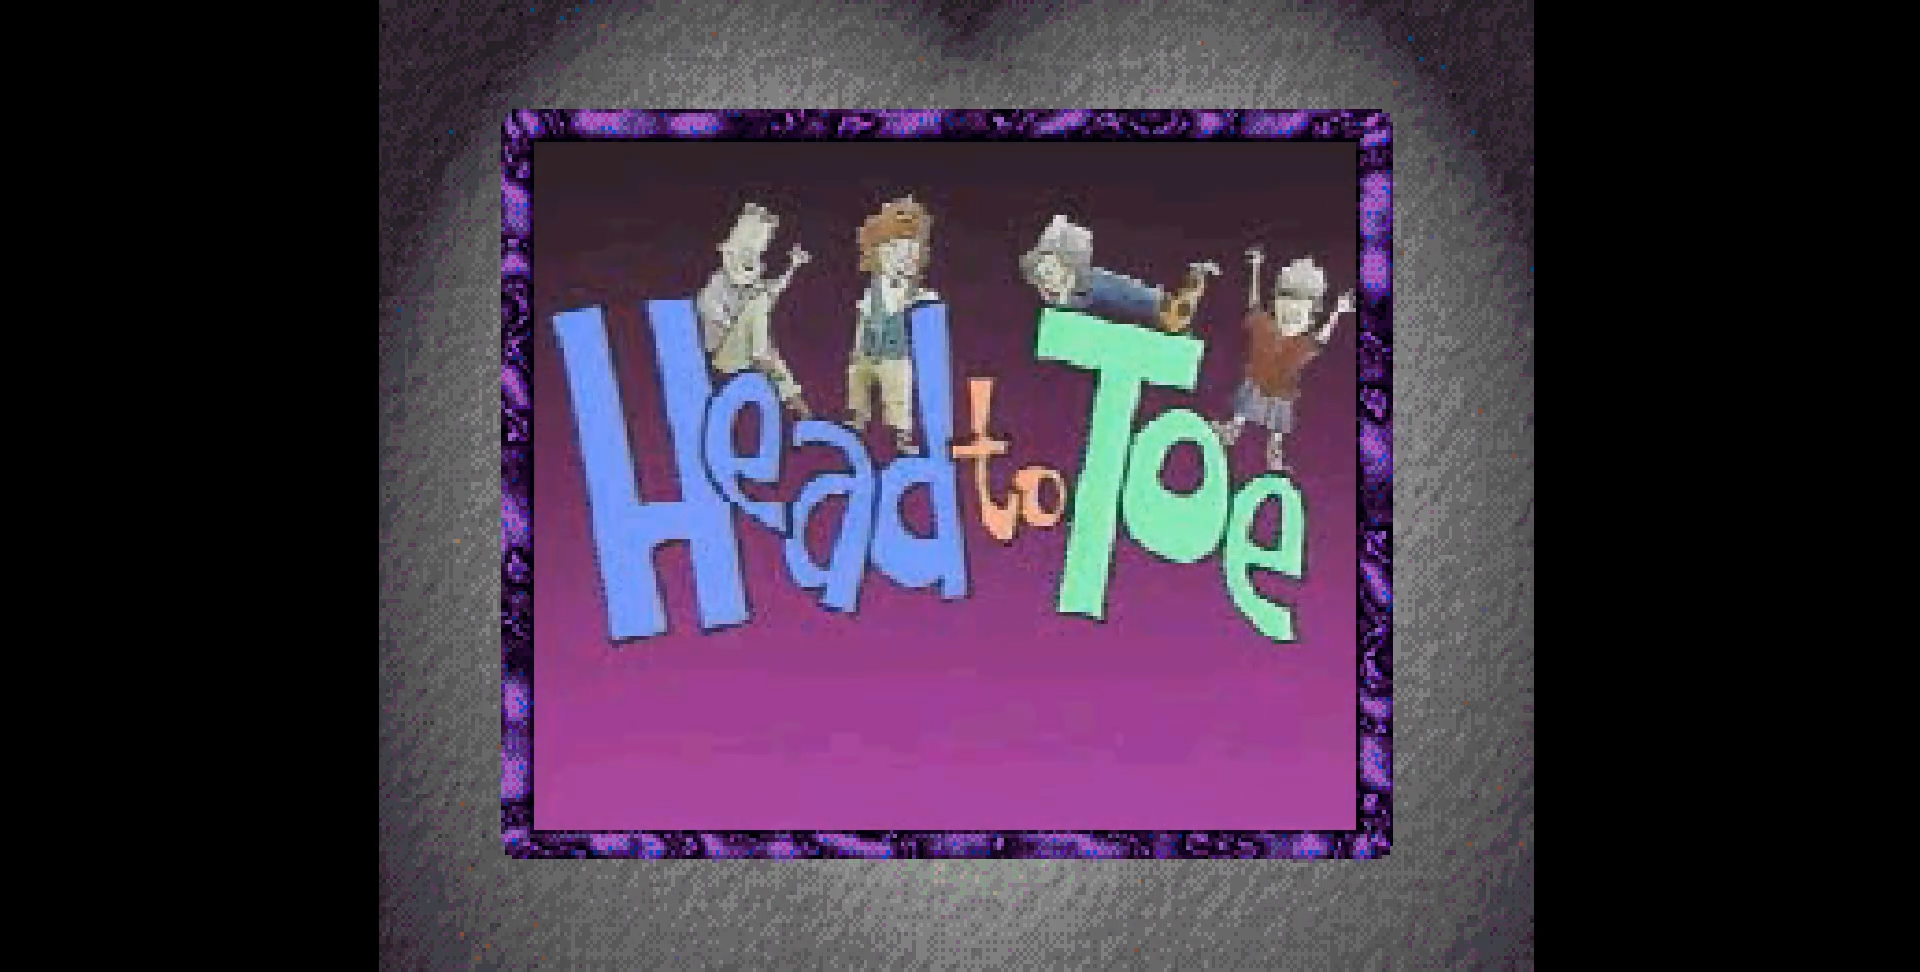
\includegraphics[width=0.5\textwidth]{./Games/HeadtoToe/Images/HeadToToeMainImage.png}
    \caption{Head To Toe Logo}
\end{figure}

Each of the videos follows a similar format: the host, Bob, is joined in the studio by a number of children who rotate in and out of the videos. Bob introduces the topic of the video, and engages the children with the material by getting them to answer questions about the topic. Within each video are sections away from the studio involving the children on-location, where they learn about the topic in a more hands-on way. The episode "A Healthy Smile" from Head To Toe 4, for example, features one of the children at a dentist's office, learning about the importance of brushing and flossing while having their teeth cleaned.

In addition, many of the episode contain additional segments related to the science topic which don't involve the children, and which may simply include a voice-over or a demonstration by Bob himself. Many of these other video segments include songs and music, which are designed to help the children remember the material, sung by outside singers (there are no credits attached to the songs, so it is unknown who the singers are). Finally, on occassion guests may enter the studio to help Bob and the children learn about the topic in more details - for example, in the episode "Sounds" from Head To Toe 3, Bert, a deaf man, comes in to teach the children about sign language.

At the beginning of each video there is a theme tune that is played, with the lyrics being as follows:

"When you get up in the morning and look in the mirror, you see your eyes, mouth, teeth, hair, ears and nose. Your muscles and bones give you a real good place for you to wear your clothes. You've got your lungs and stomach and brain and heart, and what we think and feel's a very important part of how we're put together, why we do what we do, why I look like me, and you look like you. It's a bunch of neat stuff that's fun to know, watch, listen and learn with Head To Toe."

The final note to add is that in many of the videos, the credits are incredibly lacking. There is no mention of the children involved in the production, or even who Bob is specifically. On occassion, a special thanks section is added, which may include the external people included within the video, such as an audiologist or a dentist. For every video however, there is mention to Frey Scientific, Inc, and Deonyer-Geppert Science Company, two companies which produce educational science equipment for use teaching and education.

There is very little information available about the Head To Toe series, and it is unknown how well the series was received by schools and teachers. The only material I was able to find on this series was from the YouTube channel [Inhalants For Christ](https://www.youtube.com/@volcelgaming), a channel which has uploaded all four of the disks in full, as well as a number of other Lightspan and video game titles.